% \lstdefinelanguage{json}{
%   basicstyle=\ttfamily\small,
%   commentstyle=\color{green!60!black},
%   keywordstyle=\color{blue},
%   stringstyle=\color{black},
%   showstringspaces=false,
%   breaklines=true,
%   frame=lines,
%   backgroundcolor=\color{gray!5},
% }

% \chapter{Tecnologie Infrastruttura}
% \label{cha:tecnologie_infrastruttura}


% Quando un utente di Builtdifferent preme il pulsante ``Genera ricetta personalizzata'', dietro le quinte si attiva una complessa catena di eventi che attraversa continenti e datacenter. In pochi secondi, l'applicazione mobile comunica con database in Europa, invoca funzioni serverless che orchestrano modelli di intelligenza artificiale, e restituisce una ricetta su misura completa di valori nutrizionali e istruzioni passo-passo. Questo capitolo solleva il velo su questa infrastruttura, spiegando le scelte tecnologiche che rendono possibile la ``cucina generativa'' in modo scalabile, sicuro ed economicamente sostenibile.

% Prima di entrare nel dettaglio del funzionamento del sistema, è necessario introdurre le tecnologie principali che costituiscono il cuore dell'architettura: l'ecosistema AWS con particolare focus sui servizi serverless e Supabase. Questa panoramica fornirà al lettore un inquadramento tecnico di base, utile per comprendere le scelte architetturali effettuate e le modalità con cui vengono gestiti l'elaborazione AI, le funzioni serverless e la sicurezza dei dati.

% \medskip

% \section{Supabase: Backend-as-a-Service per applicazioni moderne}
% \label{sec:supabase}

% \begin{figure}[H]
% 	\centering
% 	
\includegraphics[width=0.6\linewidth]{Images/supabase}
% 	\caption{Logo di Supabase Inc.}
% 	\label{fig:supabase_logo}
% \end{figure}

% \subsection{Panoramica generale}
% \label{subsec:supabase_overview}

% L'architettura di Supabase~\cite{supabase} si distacca dalle logiche dei BaaS (Backend as a service) tradizionali (come Firebase) puntando sull'integrazione di strumenti open-source consolidati, in primis PostgreSQL. Mentre molte soluzioni BaaS si appoggiano su database NoSQL, Supabase valorizza la maturità del modello relazionale per assicurare integrità e persistenza dei dati. Questo paradigma tecnologico è orientato a fornire agli sviluppatori uno strumento potente ma privo di limitazioni proprietarie, assicurando la piena portabilità del database e l'accesso a tutte le funzionalità avanzate del mondo SQL.

% L'ecosistema di Supabase si fonda su un'integrazione sinergica di moduli progettati per coprire l'intero ciclo di vita di un'applicazione moderna. Al centro di questa architettura risiede il database PostgreSQL, che non solo gestisce dati relazionali e complessi (come JSONB o array), ma funge da base per la generazione automatica di interfacce API (REST e GraphQL) e per il sistema di autenticazione multi-provider basato su standard JWT \cite{jwt_token}. A completare l'offerta, la piattaforma abilita la sincronizzazione dei dati in tempo reale tramite websocket e la gestione di file binari mediante un servizio di Storage integrato. La logica di business viene infine decentralizzata attraverso le Edge Functions serverless. Tale coesione architetturale solleva lo sviluppatore dall'onere di configurare infrastrutture eterogenee, ottimizzando drasticamente i tempi di go-to-market e la manutenzione operativa.

% \subsubsection{Supabase Studio: ecosistema di gestione e monitoraggio}
% Il controllo operativo dell'intera infrastruttura è affidato a Supabase Studio, un'interfaccia web centralizzata concepita per semplificare le attività di manutenzione e sviluppo. Questo strumento permette di agire direttamente sul database attraverso un editor SQL integrato, facilitando non solo la manipolazione dello schema ma anche la definizione granulare delle politiche di sicurezza tramite le Row Level Security (RLS). Oltre alla gestione dei dati, lo Studio abilita il monitoraggio delle performance e delle query in tempo reale, offrendo una panoramica completa sui log di sistema e sulle metriche di consumo. L'amministrazione degli utenti, la configurazione dei ruoli e il ciclo di vita delle Edge Functions (dal testing al deployment) vengono così unificati in un unico ambiente. Sebbene esterno alla logica applicativa pura, tale pannello si rivela indispensabile nelle fasi di ottimizzazione e debugging, elevando sensibilmente lo standard della developer experience.

% \begin{figure}[H]
% 	\centering
% 	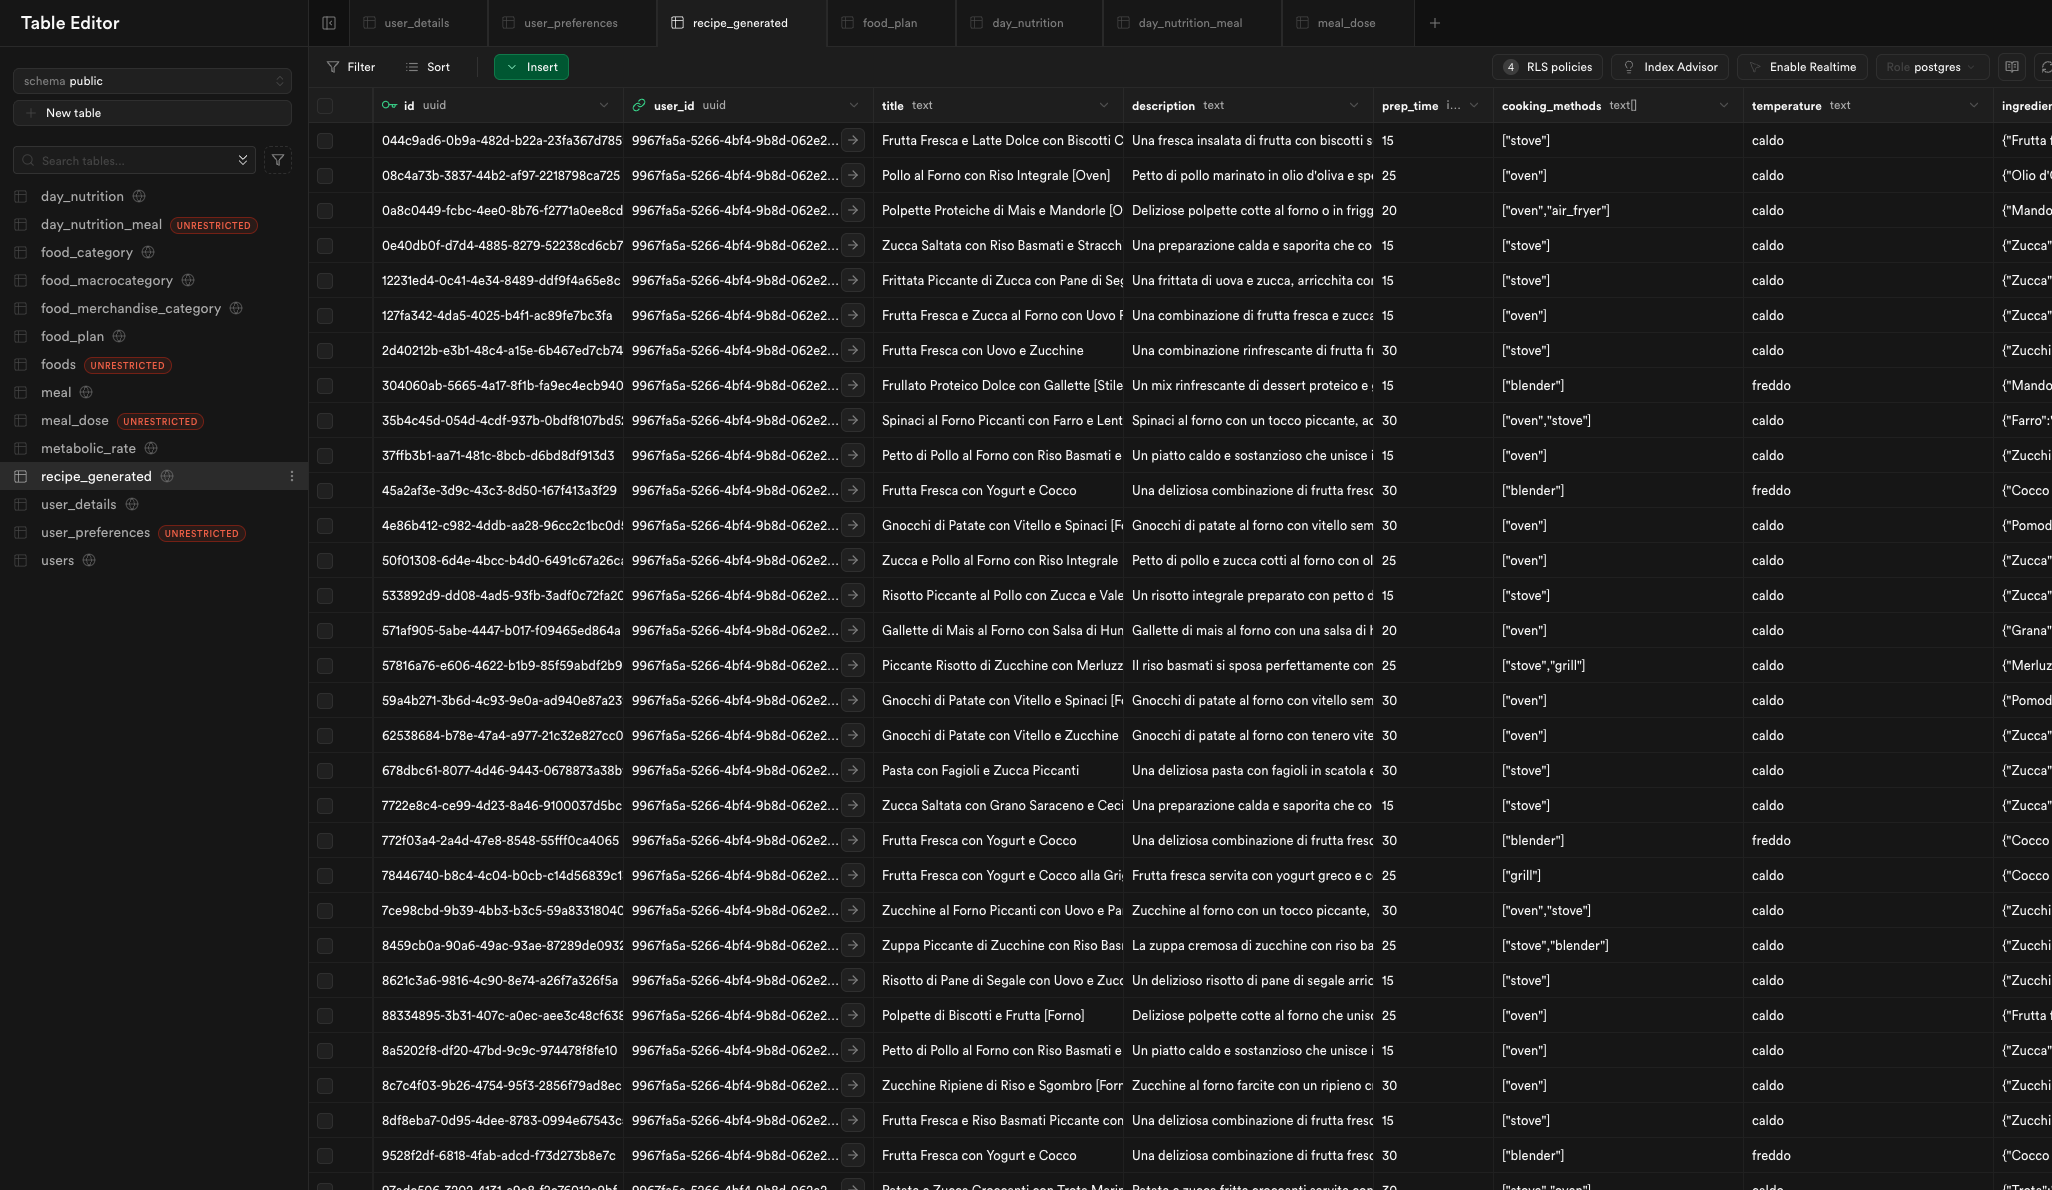
\includegraphics[width=1\linewidth]{Images/supabase_studio.png}
% 	\caption{Interfaccia di Supabase Studio per la gestione visuale del database e dei servizi.}
% 	\label{fig:supabase_studio}
% \end{figure}

% \subsection{PostgreSQL: fondamenta relazionali solide}
% \label{subsec:supabase_postgresql}

% L'intera impalcatura tecnologica di Supabase poggia su PostgreSQL, un sistema di gestione di database relazionali (RDBMS) che rappresenta lo stato dell'arte del software open-source. Sviluppato inizialmente nel 1986 presso l'Università di Berkeley e divenuto di pubblico dominio dieci anni dopo, questo motore ha saputo evolversi mantenendo una stabilità ferrea pur introducendo innovazioni avanguardistiche.

% La vera forza di PostgreSQL risiede nella sua natura ibrida. Da un lato, assicura il rispetto rigoroso delle proprietà ACID (atomicità, consistenza, isolamento e durabilità), indispensabili per l'integrità dei dati nelle operazioni più delicate. Dall'altro, offre una flessibilità vicina ai sistemi NoSQL grazie al supporto nativo per formati semi-strutturati come il JSONB, a cui si affiancano array, tipi personalizzati e range types. L'efficienza nel recupero delle informazioni è garantita da un apparato di indicizzazione estremamente variegato, che spazia dai classici B-tree ai più complessi GiST e GIN, fondamentali per gestire ricerche testuali evolute (Full-text search) senza appoggiarsi a motori esterni.

% Uno degli aspetti più rilevanti è la sua estrema estensibilità: tramite l'integrazione di extension dedicate, il database può acquisire competenze specifiche, come il trattamento di dati geospaziali tramite PostGIS o la gestione di embedding per l'intelligenza artificiale con pg$_vector.

% All'interno dell'ecosistema Supabase, PostgreSQL abbandona il ruolo di semplice contenitore di dati per diventare il vero cuore pulsante del sistema. È il database stesso a orchestrare la logica applicativa: le Row Level Security (RLS) delegano al motore SQL il controllo granulare degli accessi, mentre lo schema delle tabelle guida la generazione automatica delle API RESTful. Attraverso l'uso sinergico di trigger, stored procedures e notifiche native, PostgreSQL coordina anche l'interazione con le Edge Functions, assicurando una coerenza architetturale che semplifica lo sviluppo e massimizza le prestazioni dell'intero stack.

% \subsection{Row Level Security (RLS): sicurezza granulare dei dati}
% \label{subsec:supabase_rls}

% Una delle caratteristiche più potenti di PostgreSQL, e per estensione di Supabase, è il supporto nativo alla \textit{Row Level Security} (RLS), un meccanismo che consente di applicare controlli di accesso direttamente a livello di singola riga. Questo approccio rappresenta un’evoluzione rispetto ai modelli tradizionali di autorizzazione, nei quali i permessi vengono concessi a livello di tabella o di ruolo. Con RLS, invece, il database è in grado di valutare dinamicamente quali specifiche righe possano essere visualizzate o modificate da un determinato utente, introducendo un livello di granularità molto più fine.

% In un’architettura moderna, specialmente in scenari multi-tenant, più utenti condividono le stesse strutture dati. Senza un meccanismo di isolamento a livello di riga, l’applicazione dovrebbe occuparsi manualmente di filtrare ogni query, aumentando la complessità e il rischio di errori. RLS sposta questa responsabilità nel motore del database, garantendo che le restrizioni di accesso siano applicate in modo coerente e sistematico, indipendentemente dal codice applicativo che esegue la query.

% \subsubsection{Principi di funzionamento}

% L’attivazione della Row Level Security avviene esplicitamente su ciascuna tabella tramite il comando:

% \begin{lstlisting}[language=SQL]
% ALTER TABLE nome_tabella 
% ENABLE ROW LEVEL SECURITY;
% \end{lstlisting}

% Una volta abilitata, la tabella non espone più automaticamente tutte le proprie righe ai ruoli che dispongono dei privilegi SQL tradizionali. Diventa necessario definire delle policy che descrivano le condizioni logiche in base alle quali una riga può essere letta, inserita, modificata o eliminata. Tali condizioni sono espresse come predicati booleani e vengono valutate dal database per ogni operazione eseguita sulla tabella.

% Nel contesto di Supabase, le policy possono fare riferimento all’identità dell’utente autenticato attraverso funzioni come \texttt{auth.uid()}, che restituisce l’identificativo dell’utente associato al token JWT fornito dal sistema di autenticazione. In questo modo, il controllo di accesso diventa sensibile al contesto della richiesta e non dipende esclusivamente dal ruolo statico associato alla connessione al database.

% \subsubsection{Esempio pratico di policy RLS}

% Si consideri una tabella che memorizza le preferenze degli utenti e che contiene un campo \texttt{user\_id} per identificare il proprietario di ciascuna riga. Per garantire che ogni utente possa accedere esclusivamente ai propri dati, è possibile definire la seguente configurazione:

% \begin{lstlisting}[language=SQL, caption=Esempio di policy RLS per accesso esclusivo ai propri dati, label=lst:rls_preferences]
% -- Abilitazione RLS sulla tabella
% ALTER TABLE user_preferences 
% ENABLE ROW LEVEL SECURITY;

% -- Policy per la lettura
% CREATE POLICY "Utenti vedono solo le proprie preferenze"
% ON user_preferences
% FOR SELECT
% USING (user_id = auth.uid());

% \end{lstlisting}
% In questo scenario, ogni operazione di lettura sulla tabella viene automaticamente filtrata dal motore PostgreSQL in base alla condizione specificata nella clausola \texttt{USING}. Anche se l’applicazione eseguisse una query priva di clausole \texttt{WHERE}, il database restituirebbe esclusivamente le righe per cui \texttt{user\_id} coincide con l’identificativo dell’utente autenticato. Questo comportamento riduce drasticamente il rischio di accessi indebiti dovuti a errori logici o a dimenticanze nel codice dell’applicazione.
% \subsubsection{Vantaggi architetturali di RLS}

% L’adozione della Row Level Security produce effetti rilevanti sul piano architetturale. Innanzitutto, introduce un principio di \textit{security by design}, poiché le regole di autorizzazione vengono dichiarate e fatte rispettare direttamente dal database. In secondo luogo, semplifica il livello applicativo, che non deve più replicare la logica di filtraggio in ogni endpoint o servizio. Questo favorisce una separazione più netta tra logica di business e controllo degli accessi.

% Dal punto di vista della multi-tenancy, RLS consente di utilizzare un unico schema condiviso mantenendo un isolamento rigoroso dei dati. Le policy sono espresse in forma dichiarativa e possono essere revisionate, versionate e sottoposte ad audit con maggiore facilità rispetto a controlli distribuiti nel codice applicativo. Inoltre, poiché le condizioni RLS vengono integrate nel processo di pianificazione delle query, PostgreSQL può ottimizzarne l’esecuzione, mantenendo prestazioni adeguate anche in presenza di regole di accesso articolate.

% \begin{figure}[H]
% 	\centering
% 	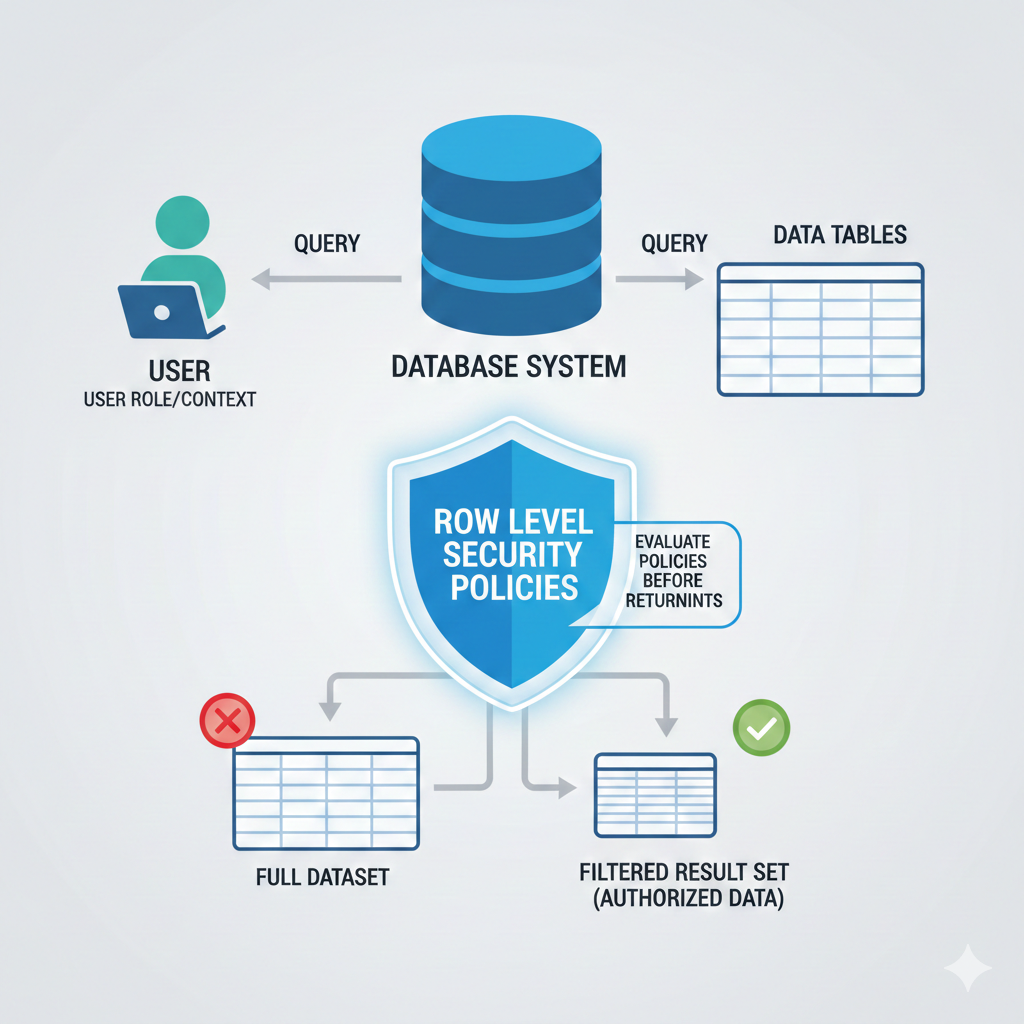
\includegraphics[width=0.7\linewidth]{Images/rls_schema.png}
% 	\caption{Diagramma concettuale di Row Level Security: le policy vengono valutate dal database prima di restituire i risultati.}
% 	\label{fig:rls_diagram}
% \end{figure}

% \subsection{Edge Functions: computazione distribuita e serverless}
% \label{subsec:supabase_edge_functions}

% Le \textit{Edge Functions} \cite{supabase_edge_functions} di Supabase rappresentano un ambiente di esecuzione serverless basato su Deno~\cite{deno}, un runtime moderno per JavaScript e TypeScript progettato per superare alcune limitazioni architetturali di Node.js. A differenza delle tradizionali funzioni serverless eseguite in data center centralizzati, le Edge Functions vengono distribuite su una rete globale di edge node, avvicinando l'elaborazione all'utente finale e riducendo drasticamente la latenza.

% \subsubsection{Architettura e modello di esecuzione}

% Le Edge Functions si basano su \textit{V8 isolates}, la stessa tecnologia utilizzata dai browser moderni per isolare l'esecuzione del codice JavaScript. Questo approccio permette un avvio quasi istantaneo (ordine dei millisecondi) con un overhead di memoria estremamente ridotto rispetto ai container tradizionali, abilitando una scalabilità orizzontale praticamente illimitata.

% Caratteristiche principali del modello di esecuzione:

% \begin{itemize}
%     \item \textbf{Cold start minimale}: le funzioni si avviano in pochi millisecondi senza i tempi di boot tipici dei container;
%     \item \textbf{Distribuzione geografica}: il codice viene replicato automaticamente su centinaia di edge location nel mondo;
%     \item \textbf{Scalabilità automatica}: il sistema scala in base al carico senza configurazione manuale;
%     \item \textbf{Integrazione nativa}: accesso diretto al database Supabase tramite JWT e client SDK ottimizzati;
%     \item \textbf{TypeScript nativo}: supporto first-class per TypeScript senza necessità di transpilazione separata.
% \end{itemize}

% \subsubsection{Casi d'uso tipici}

% Le Edge Functions sono particolarmente adatte per implementare logiche che beneficiano di bassa latenza e alta disponibilità:

% \begin{itemize}
%     \item validazione e trasformazione di dati in ingresso prima della persistenza;
%     \item orchestrazione di chiamate a API esterne (es. servizi AI, payment gateway);
%     \item generazione dinamica di contenuti personalizzati;
%     \item implementazione di webhook e integrazioni real-time;
%     \item logiche di business complesse che non possono essere espresse tramite SQL.
% \end{itemize}

% \subsection{Modello dati e struttura relazionale}

% Il sistema si basa su uno schema PostgreSQL progettato per gestire in modo efficiente la gerarchia dei dati nutrizionali e le preferenze utente. La struttura a cascata permette al nutrizionista di definire piani alimentari dettagliati, che vengono poi utilizzati come base per la generazione personalizzata delle ricette.

% \paragraph{Piano nutrizionale gerarchico}

% La struttura dati per i piani nutrizionali si articola su tre livelli:

% \begin{enumerate}
%     \item \textbf{day\_nutrition}: rappresenta la configurazione giornaliera, includendo il bilanciamento dei macronutrienti (proteine, lipidi, carboidrati) e eventuali note su integrazioni o pasti liberi;
%     \item \textbf{day\_nutrition\_meal}: definisce la distribuzione dei macronutrienti per ogni singolo pasto della giornata (colazione, pranzo, cena, spuntini);
%     \item \textbf{meal\_dose}: specifica gli alimenti concreti, le quantità e le modalità di preparazione per ciascun pasto.
% \end{enumerate}

% Questa organizzazione permette una flessibilità estrema nella definizione dei piani, consentendo al nutrizionista di personalizzare ogni aspetto del regime alimentare mantenendo coerenza e tracciabilità.

% \begin{table}[H]
% \centering
% \caption{Struttura tabella \texttt{day\_nutrition}: configurazione giornaliera del piano nutrizionale}
% \label{tab:day_nutrition}
% \begin{tabular}{|l|l|p{6cm}|}
% \hline
% \textbf{Colonna} & \textbf{Tipo} & \textbf{Note} \\
% \hline
% id & UUID PK & Identificativo unico della configurazione giornaliera \\
% \hline
% created\_at & TIMESTAMPTZ & Data e ora di creazione \\
% \hline
% food\_plan & UUID & Riferimento al piano alimentare principale \\
% \hline
% day & SMALLINT & Numero del giorno nel piano (1-7, 1-14, etc.) \\
% \hline
% integration & TEXT & Note su eventuali integrazioni suggerite \\
% \hline
% free\_meals & TEXT & Indicazioni su pasti liberi concessi \\
% \hline
% pro\_gr & INTEGER & Proteine totali giornaliere in grammi \\
% \hline
% lip\_gr & INTEGER & Lipidi totali giornalieri in grammi \\
% \hline
% cho\_gr & INTEGER & Carboidrati totali giornalieri in grammi \\
% \hline
% \end{tabular}
% \end{table}

% \begin{table}[H]
% \centering
% \caption{Struttura tabella \texttt{day\_nutrition\_meal}: distribuzione macronutrienti per pasto}
% \label{tab:day_nutrition_meal}
% \begin{tabular}{|l|l|p{6cm}|}
% \hline
% \textbf{Colonna} & \textbf{Tipo} & \textbf{Note} \\
% \hline
% id & UUID PK & Identificativo unico del pasto \\
% \hline
% day\_nutrition & UUID & Riferimento alla configurazione giornaliera \\
% \hline
% meal & TEXT & Tipologia di pasto (colazione, pranzo, cena, spuntino) \\
% \hline
% pro\_gr & INTEGER & Proteine previste per questo pasto in grammi \\
% \hline
% lip\_gr & INTEGER & Lipidi previsti per questo pasto in grammi \\
% \hline
% cho\_gr & INTEGER & Carboidrati previsti per questo pasto in grammi \\
% \hline
% \end{tabular}
% \end{table}

% \begin{table}[H]
% \centering
% \caption{Struttura tabella \texttt{meal\_dose}: alimenti specifici e quantità}
% \label{tab:meal_dose}
% \begin{tabular}{|l|l|p{6cm}|}
% \hline
% \textbf{Colonna} & \textbf{Tipo} & \textbf{Note} \\
% \hline
% id & UUID PK & Identificativo unico della dose \\
% \hline
% food & UUID & Riferimento all'alimento nel database nutrizionale \\
% \hline
% quantity & SMALLINT & Quantità in grammi dell'alimento \\
% \hline
% split & BOOLEAN & Indica se l'alimento può essere diviso in più porzioni \\
% \hline
% day\_nutrition\_meal & UUID & Riferimento al pasto di appartenenza \\
% \hline
% \end{tabular}
% \end{table}

% \paragraph{Preferenze utente e questionario iniziale}

% Le preferenze dell'utente vengono raccolte tramite un questionario strutturato eseguito prima della prima generazione di ricette. Queste informazioni includono attrezzature disponibili in cucina, allergie, intolleranze, preferenze culinarie e vincoli di tempo.

% \begin{table}[H]
% \centering
% \caption{Struttura tabella \texttt{user\_preferences}: preferenze e vincoli utente}
% \label{tab:user_preferences}
% \begin{tabular}{|l|l|p{6cm}|}
% \hline
% \textbf{Colonna} & \textbf{Tipo} & \textbf{Note} \\
% \hline
% id & UUID PK & Identificativo unico delle preferenze \\
% \hline
% user\_id & UUID UNIQUE & Riferimento all'utente (auth.users) \\
% \hline
% cooking\_equipment & TEXT[] & Array di attrezzature disponibili in cucina \\
% \hline
% created\_at & TIMESTAMPTZ & Data di creazione del profilo \\
% \hline
% updated\_at & TIMESTAMPTZ & Data ultimo aggiornamento (trigger automatico) \\
% \hline
% \end{tabular}
% \end{table}

% L'utilizzo di array PostgreSQL (\texttt{TEXT[]}) per memorizzare le attrezzature disponibili permette query efficienti e flessibilità nell'aggiornamento delle preferenze senza necessità di tabelle di join aggiuntive.

% \paragraph{Ricette generate e feedback}

% Ogni ricetta generata dal sistema AI viene persistita nel database insieme ai metadati nutrizionali, agli ingredienti utilizzati e alle informazioni di preparazione. La tabella \texttt{recipe\_generated} sfrutta il tipo JSONB di PostgreSQL per memorizzare strutture complesse come ingredienti dettagliati e condimenti suggeriti.

% \begin{table}[H]
% \centering
% \caption{Struttura tabella \texttt{recipe\_generated}: ricette create dal sistema AI}
% \label{tab:recipe_generated}
% \small
% \begin{tabular}{|l|l|p{5.5cm}|}
% \hline
% \textbf{Colonna} & \textbf{Tipo} & \textbf{Note} \\
% \hline
% id & UUID PK & Identificativo unico della ricetta \\
% \hline
% user\_id & UUID & Proprietario della ricetta \\
% \hline
% title & TEXT & Titolo della ricetta (obbligatorio) \\
% \hline
% description & TEXT & Descrizione e note preparazione \\
% \hline
% prep\_time & INTEGER & Tempo preparazione in minuti \\
% \hline
% cooking\_methods & TEXT[] & Metodi cottura utilizzati \\
% \hline
% temperature & TEXT & Temperatura servizio (caldo/freddo/ambiente) \\
% \hline
% ingredients & JSONB & Ingredienti dettagliati con quantità \\
% \hline
% calories & INTEGER & Calorie totali del piatto \\
% \hline
% tastes & TEXT[] & Profili gustativi (dolce, salato, speziato, etc.) \\
% \hline
% suggested\_seasonings & JSONB & Condimenti consigliati \\
% \hline
% unused\_ingredients & JSONB & Ingredienti del piano non utilizzati \\
% \hline
% feedback\_rating & TEXT & Valutazione utente (sad/neutral/happy) \\
% \hline
% feedback\_notes & TEXT & Note feedback testuale \\
% \hline
% feedback\_date & TIMESTAMPTZ & Data invio feedback \\
% \hline
% is\_favorite & BOOLEAN & Ricetta contrassegnata come preferita \\
% \hline
% created\_at & TIMESTAMPTZ & Data creazione ricetta \\
% \hline
% updated\_at & TIMESTAMPTZ & Data ultimo aggiornamento \\
% \hline
% \end{tabular}
% \end{table}

% \subsubsection{Indicizzazione strategica per performance}

% Per garantire tempi di risposta rapidi anche con volumi crescenti di ricette, sono stati creati indici mirati sulle colonne più frequentemente interrogate. In particolare:

% \begin{itemize}
%     \item \textbf{Indice B-tree su user\_id}: ottimizza il filtraggio delle ricette per utente, operazione eseguita in ogni richiesta;
%     \item \textbf{Indice B-tree su created\_at (DESC)}: permette ordinamento cronologico efficiente per visualizzare le ricette più recenti;
%     \item \textbf{Indice parziale su feedback\_rating}: indicizza solo le righe con feedback presente, ottimizzando le query di analisi;
%     \item \textbf{Indici GIN su array}: \texttt{cooking\_methods} e \texttt{tastes} utilizzano Generalized Inverted Index per ricerche su contenuti array;
%     \item \textbf{Indici GIN su JSONB}: \texttt{ingredients} e \texttt{suggested\_seasonings} permettono ricerche efficienti all'interno delle strutture JSON complesse.
% \end{itemize}

% L'utilizzo di indici GIN (Generalized Inverted Index) su colonne array e JSONB permette ricerche efficienti su contenuti complessi, come trovare tutte le ricette che utilizzano un determinato ingrediente o metodo di cottura, senza necessità di scansioni complete della tabella.

% \subsubsection{Scalabilità e performance}

% L'architettura basata su Supabase offre vantaggi significativi in termini di scalabilità:

% \begin{itemize}
%     \item \textbf{Scalabilità del database}: PostgreSQL permette scaling verticale (CPU, RAM) e read replicas per distribuire il carico di lettura;
%     \item \textbf{Edge Functions distribuite}: l'esecuzione geograficamente distribuita riduce la latenza per utenti in diverse aree geografiche;
%     \item \textbf{Connection pooling nativo}: Supabase implementa PgBouncer per gestire efficientemente migliaia di connessioni concorrenti;
%     \item \textbf{Caching intelligente}: le query frequenti vengono cachate automaticamente a livello edge;
%     \item \textbf{Auto-scaling delle funzioni}: le Edge Functions scalano automaticamente in base al numero di richieste.
% \end{itemize}

% Questo modello permette al sistema di gestire picchi di traffico senza degradazione delle performance, caratteristica fondamentale per un'applicazione consumer-facing.

% \subsubsection{Integrazione con intelligenza artificiale}

% Le Edge Functions rappresentano il punto di integrazione ideale con i servizi di AI generativa utilizzati per creare le ricette. Il flusso tipico prevede:

% \begin{enumerate}
%     \item L'utente richiede la generazione di una nuova ricetta;
%     \item La Edge Function recupera i dati nutrizionali dal piano del nutrizionista e le preferenze utente;
%     \item I dati vengono strutturati in un prompt ottimizzato per il modello AI;
%     \item Il modello genera la ricetta rispettando vincoli nutrizionali e preferenze;
%     \item La Edge Function valida la risposta e la persiste tramite \texttt{save\_recipe};
%     \item La ricetta viene restituita all'utente e resa disponibile per feedback futuro.
% \end{enumerate}

% Questo approccio mantiene la logica di orchestrazione AI centralizzata e sicura nel backend, evitando di esporre chiavi API o logiche sensibili nel client.

% % \begin{figure}[H]
% % 	\centering
% % 	\includegraphics[width=1\linewidth]{Images/ai_integration_flow}
% % 	\caption{Flusso di integrazione tra Edge Functions, database Supabase e servizi AI per la generazione ricette.}
% % 	\label{fig:ai_integration}
% % \end{figure}

% \subsection{Considerazioni finali}

% L'adozione di Supabase come piattaforma backend ha permesso di costruire un sistema robusto, sicuro e scalabile con tempi di sviluppo significativamente ridotti rispetto a un'architettura tradizionale self-hosted. La combinazione di PostgreSQL, Row Level Security ed Edge Functions fornisce una base solida per implementare logiche complesse mantenendo al contempo semplicità operativa e controllo granulare sui dati.

% La scelta di un'architettura open-source evita vendor lock-in e garantisce la possibilità di migrare l'infrastruttura su deployment self-hosted in futuro, se necessario, mantenendo piena compatibilità con lo stack tecnologico esistente.

% \section{AWS (Amazon Web Services)}

% \begin{figure}[H]
% 	\centering
% 	
\includegraphics[width=0.6\linewidth]{Images/aws.png}
% 	\caption{Logo di Amazon Web Services}
% 	\label{fig:aws_logo}
% \end{figure}

% \subsection{La Scelta del Cloud Provider}

% Amazon Web Services (AWS)~\cite{aws} rappresenta la piattaforma cloud leader a livello globale, lanciata da Amazon nel 2006. Con oltre 200 servizi completi disponibili da datacenter distribuiti in tutto il mondo, AWS offre un ecosistema completo per la costruzione, deployment e gestione di applicazioni di qualsiasi scala e complessità.

% La scelta di AWS come backbone infrastrutturale per il sistema di Cucina Generativa non è stata casuale. Quando il team di Builtdifferent ha iniziato a progettare il sistema di generazione ricette, si è trovato di fronte a un dilemma comune nelle startup tecnologiche: come costruire qualcosa che funzioni oggi con risorse limitate, ma che possa scalare domani senza riscrivere tutto da zero? Il modello di business di AWS basato sul \emph{pay-as-you-go} ha rappresentato la risposta ideale a questa sfida. Gli utenti pagano solo per le risorse effettivamente consumate, senza costi fissi iniziali o impegni a lungo termine. Questo approccio ha democratizzato l'accesso a infrastrutture enterprise, rendendole disponibili anche per startup e piccoli team.

% Nel contesto di questa tesi, AWS non è stato scelto solo per la sua maturità e affidabilità comprovate nel tempo, ma soprattutto per la sua offerta integrata di servizi serverless e di intelligenza artificiale che si allineano perfettamente con i requisiti del sistema: scalabilità automatica in risposta ai picchi di traffico, controllo granulare dei costi operativi, sicurezza avanzata per la protezione dei dati sensibili degli utenti, e accesso immediato a modelli AI di ultima generazione senza la necessità di gestire infrastruttura GPU complessa.

% \subsection{Il Paradigma Serverless: Un Cambio di Mentalità}

% Il \emph{serverless computing} su AWS rappresenta un cambio di paradigma rispetto alle architetture tradizionali basate su server. Per comprenderne il valore, è utile fare un passo indietro. Tradizionalmente, lanciare un'applicazione web significava stimare quanti server comprare o affittare: troppo pochi e l'applicazione crasha sotto carico nei momenti di picco, troppi e si sprecano soldi in macchine che stanno al cinque percento di utilizzo per la maggior parte del tempo. Ogni decisione di scaling richiedeva giorni o settimane di pianificazione, acquisto hardware, configurazione e deployment.

% Con il serverless, questo problema semplicemente non esiste più. Invece di provisioning, gestione e scaling manuale di macchine virtuali o container, lo sviluppatore si concentra esclusivamente sulla logica di business, mentre AWS gestisce automaticamente l'infrastruttura sottostante. L'applicazione si adatta istantaneamente al carico, scalando da zero a migliaia di istanze concorrenti in pochi secondi, per poi tornare a zero quando non c'è traffico.

% I due pilastri del nostro sistema serverless sono AWS Lambda e API Gateway, che lavorano in perfetta sinergia per gestire il flusso di richieste dall'utente finale fino all'intelligenza artificiale generativa.

% \subsubsection{AWS Lambda: Computing Senza Server}

% AWS Lambda~\cite{lambda} è il servizio di computing serverless che esegue codice in risposta a eventi senza richiedere il provisioning o la gestione di server. Il codice, organizzato in unità chiamate ``funzioni'', viene eseguito in un ambiente altamente disponibile, con scaling automatico e billing al millisecondo di esecuzione effettiva.

% Ogni funzione Lambda è essenzialmente un piccolo programma che ``dorme'' finché non viene invocato. Quando arriva una richiesta di generazione ricetta, AWS risveglia istantaneamente una copia della funzione (o ne crea una nuova se necessario), la esegue, e la spegne quando ha completato il suo compito. Il tutto in millisecondi, e si paga solo per quei millisecondi di esecuzione effettiva. Per un'applicazione come Builtdifferent, con picchi di traffico prevedibili all'ora di pranzo e cena e periodi di quiete durante la notte, questo significa un'ottimizzazione dei costi straordinaria: la capacità computazionale è disponibile esattamente quando serve, senza sprechi.

% \begin{figure}[H]
% 	\centering
% 	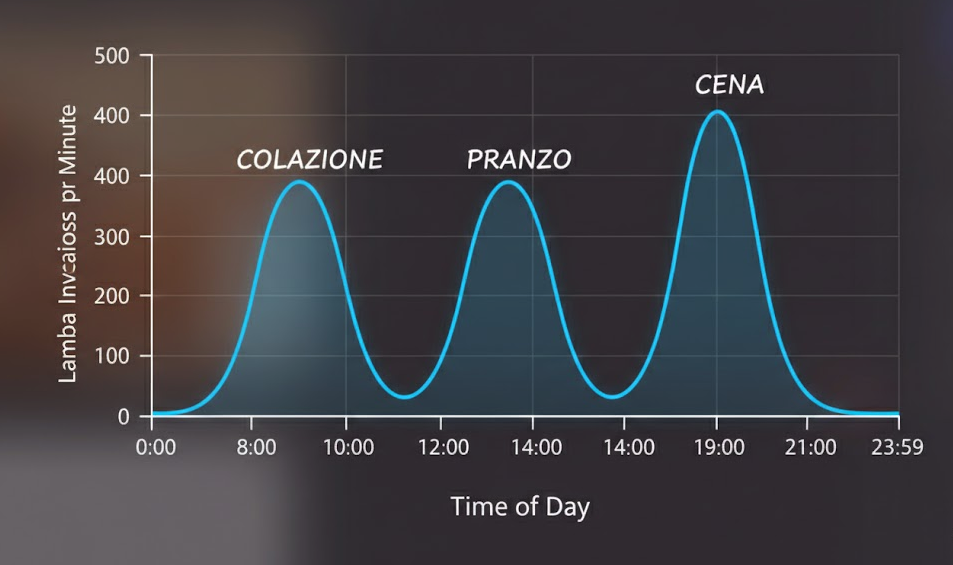
\includegraphics[width=0.8\linewidth]{Images/grafico_usage.png}
% 	\caption{Vantaggi di utilizzare un pay-as-you-go}
% 	\label{fig:aws_logo}
% \end{figure}

% Per il sistema di Cucina Generativa, Lambda è la scelta ideale perché gestisce automaticamente i picchi di traffico (ad esempio, molte richieste simultanee di ricette durante l'ora di cena) senza intervento manuale o configurazione preventiva. Il sistema addebita solo quando le funzioni sono effettivamente eseguite, eliminando i costi di idle time. Inoltre, Lambda si integra nativamente con altri servizi AWS come API Gateway per l'esposizione HTTP, Bedrock per l'intelligenza artificiale, e CloudWatch per il monitoraggio, creando un ecosistema coeso e facile da gestire. Il supporto nativo per Python facilita l'implementazione della logica AI complessa richiesta per la generazione delle ricette.

% \subsubsection{API Gateway}

% Amazon API Gateway~\cite{api-gateway} è un servizio completamente gestito per la creazione, pubblicazione, manutenzione, monitoraggio e protezione di API a qualsiasi scala. Nel nostro sistema, API Gateway funge da punto di ingresso pubblico, gestendo aspetti cruciali come l'autenticazione degli utenti tramite token JWT, il rate limiting per prevenire abusi e sovraccarichi, e il routing intelligente delle richieste verso le appropriate funzioni Lambda backend.
% L'architettura risultante è elegante nella sua semplicità: l'applicazione mobile effettua una chiamata HTTPS all'endpoint pubblico di API Gateway, che valida il token di autenticazione, verifica i limiti di utilizzo dell'utente, e inoltra la richiesta alla funzione Lambda corretta. Lambda elabora la richiesta, invoca i servizi necessari (come Bedrock per la generazione AI), e restituisce la risposta attraverso lo stesso percorso. Tutto questo avviene in pochi secondi, con un'esperienza utente fluida e senza che lo sviluppatore debba preoccuparsi di gestire server, load balancer, o certificati SSL.

% \begin{figure}[H]
% 	\centering
% 	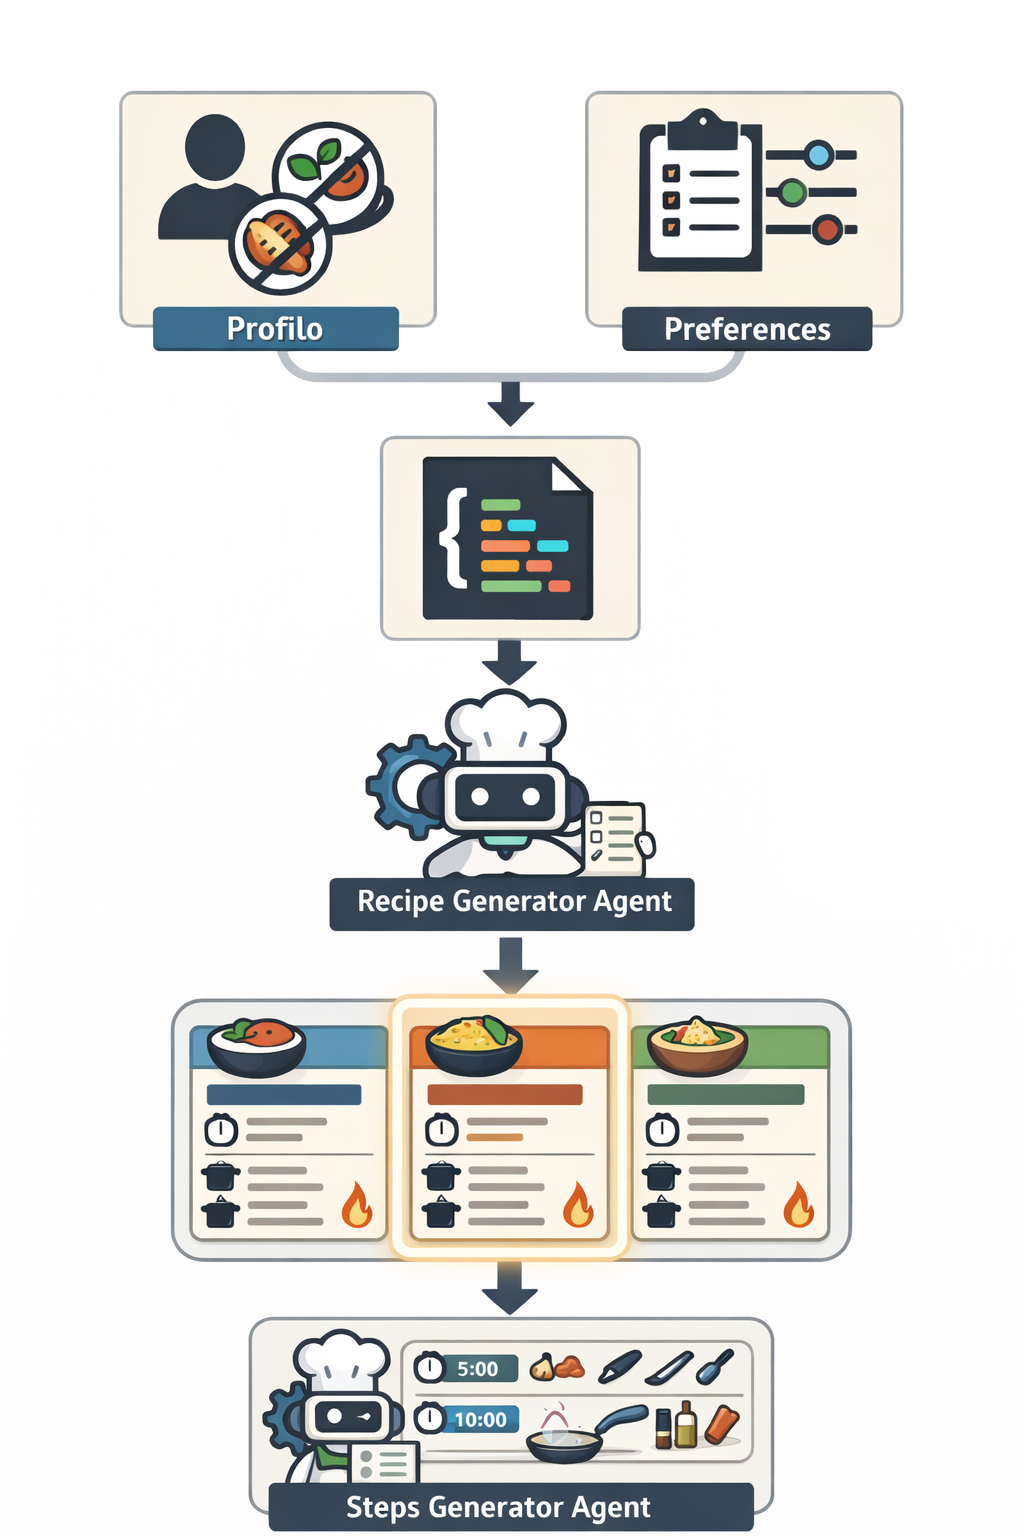
\includegraphics[width=0.85\linewidth]{Images/flusso_generazione.png}
% 	\caption{Architettura serverless semplificata: dal client mobile attraverso API Gateway fino alle funzioni Lambda}
% 	\label{fig:aws_serverless_architecture}
% \end{figure}

% \section{AWS Bedrock e i Modelli di Fondazione}
% \label{sec:aws-bedrock}

% \subsection{L'Accesso all'Intelligenza Artificiale Generativa}

% AWS Bedrock~\cite{bedrock} è un servizio completamente gestito che offre accesso attraverso un'API unificata a modelli di fondazione (\emph{Foundation Models}) di diversi fornitori leader nel settore dell'intelligenza artificiale. Lanciato nel 2023, Bedrock rappresenta la risposta di AWS al crescente bisogno delle aziende di integrare capacità generative AI nelle loro applicazioni, senza la complessità e i costi di gestire l'infrastruttura sottostante.

% Immaginiamo che un utente vegetariano con intolleranza al lattosio chieda al sistema una ricetta generata. Questa richiesta apparentemente semplice nasconde una complessità notevole: il sistema deve comprendere i limiti imposti, consultare le preferenze alimentari dell'utente salvate nel database e passarle nella query iniziale, filtrare migliaia di possibili combinazioni di ingredienti rispettando sia i vincoli nutrizionali sia quelli di gusto e appetibilità (dichiarati in un questionario previo generazione che verrà analizzato successivamente), e infine generare non solo una ricetta realistica ma anche istruzioni di cottura coerenti, dettagliate e invitanti. Tutto questo è reso possibile dai modelli di fondazione accessibili tramite Bedrock.


% \subsection{Amazon Nova Lite: La Scelta per la Cucina Generativa}
% A differenza dell'uso diretto di API pubbliche di terze parti (come quelle di OpenAI o Anthropic), Bedrock offre diversi vantaggi cruciali per un'applicazione enterprise che gestisce dati sensibili degli utenti. Innanzitutto, l'integrazione nativa con l'ecosistema AWS significa che l'accesso ai modelli è controllato tramite IAM (lo stesso sistema di permessi usato per tutti gli altri servizi AWS), i log vengono automaticamente inviati a CloudWatch per analisi e debugging, e la sicurezza di rete può essere rafforzata mantenendo il traffico all'interno di una Virtual Private Cloud. In secondo luogo, la sovranità dei dati è garantita: tutta l'elaborazione avviene all'interno dell'infrastruttura AWS, un aspetto cruciale per la compliance con normative come il GDPR. Il modello di costo è inoltre trasparente e prevedibile, senza sorprese legate al consumo. Infine, la flessibilità nel modello sottostante permette di cambiare provider AI (da un modello Amazon a uno Anthropic qualora un domani si volesse aggiungere ulteriore creatività) senza modifiche al codice applicativo, garantendo longevità all'investimento tecnologico.

% Tra i vari modelli disponibili su Bedrock, per questo progetto è stato selezionato \emph{Amazon Nova Lite} \cite{aws_nova_models}. Questa scelta è stata guidata da un'attenta analisi di costi, prestazioni e qualità dell'output.

% Il primo criterio è stato il bilanciamento costo-prestazioni. Nova Lite offre un ottimo compromesso tra qualità generativa e costo operativo per token generato, un aspetto essenziale per la sostenibilità economica di una startup in fase di crescita. Generare decine di migliaia di ricette al mese con modelli più costosi avrebbe reso il servizio economicamente insostenibile.

% Il secondo fattore determinante è stata l'ottimizzazione per la lingua italiana. Nei test comparativi condotti durante la fase di prototipazione, Nova Lite ha dimostrato una capacità superiore nella generazione di testo in lingua italiana naturale e idiomatica, rispetto ad altri modelli della stessa fascia di prezzo. Questo è un requisito fondamentale considerando che l'utenza di Builtdifferent è principalmente italiana e si aspetta ricette scritte in un italiano fluido, con terminologia culinaria corretta e istruzioni chiare.

% La bassa latenza rappresenta il terzo pilastro della scelta. I tempi di risposta di Nova Lite si attestano costantemente sotto i cinque secondi per la generazione di una ricetta completa (inclusi ingredienti, procedimento e valori nutrizionali), garantendo un'esperienza utente fluida senza frustranti attese. In un'applicazione mobile, ogni secondo di latenza può tradursi in abbandono da parte dell'utente.

% Infine, la conformità nativa con l'ecosistema AWS semplifica enormemente la gestione degli accessi tramite IAM, il monitoraggio delle performance tramite CloudWatch, e l'implementazione di politiche di sicurezza granulari, aspetti che verranno approfonditi nelle sezioni successive.

% \begin{figure}[H]
% 	\centering
% 	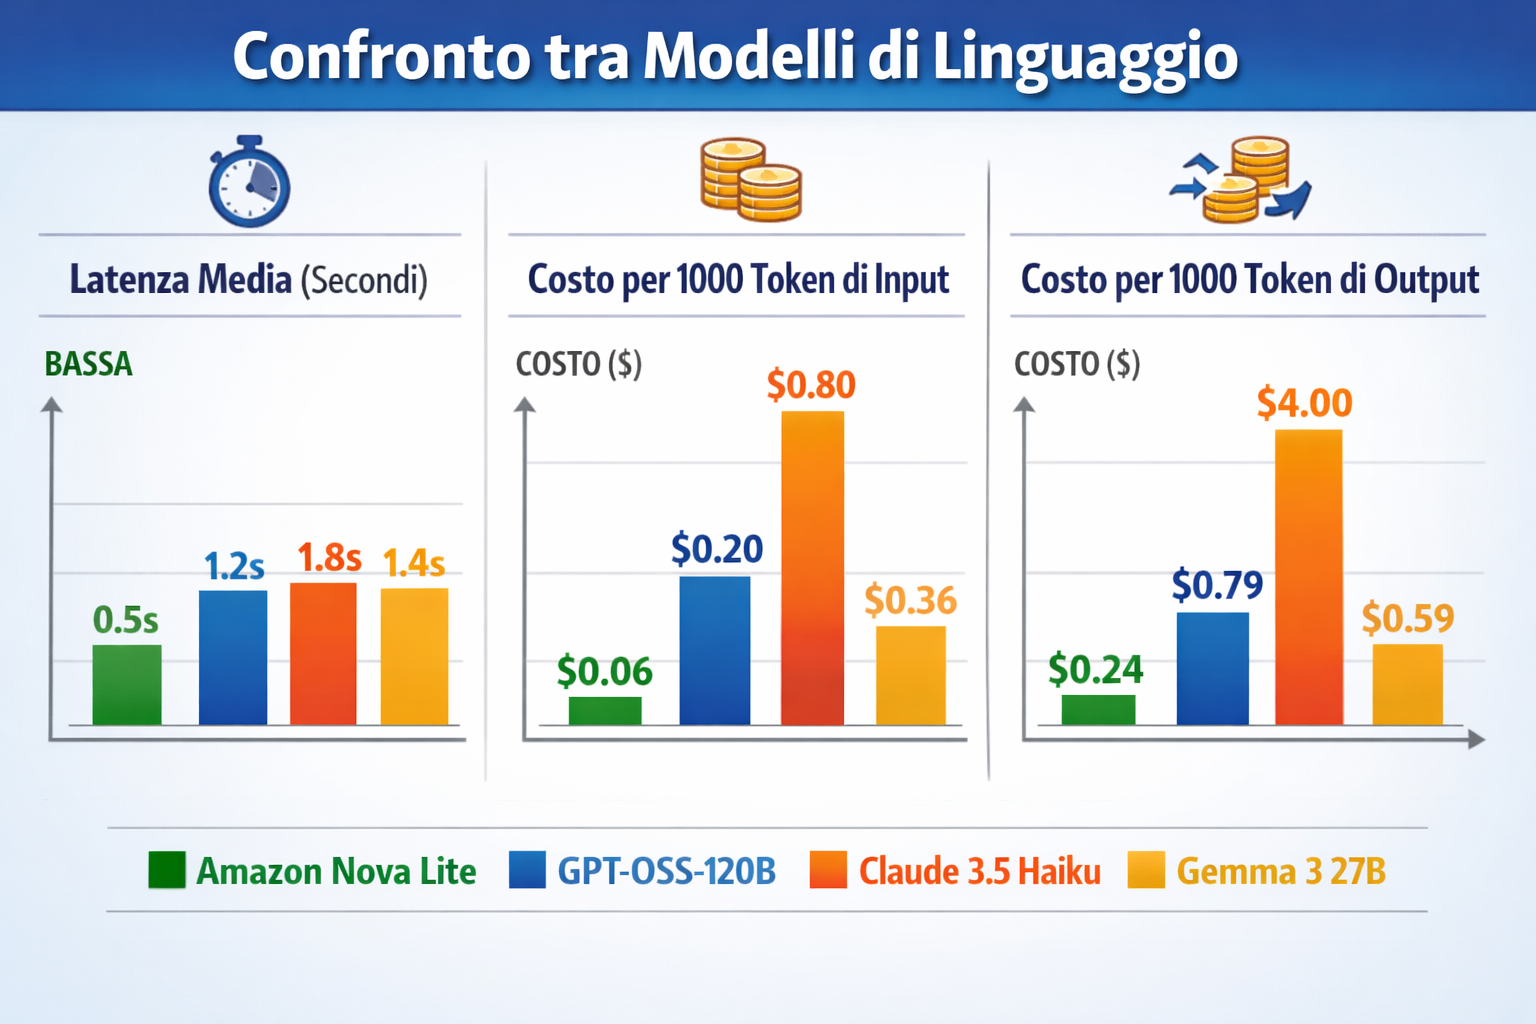
\includegraphics[width=0.85\linewidth]{Images/pricing_comparison.png}
% 	\caption{Comparazione costi e latenza tra i diversi modelli}
% 	\label{fig:aws_serverless_architecture}
% \end{figure}

% \subsection{Agenti Bedrock: Specializzazione e Controllo}

% Bedrock supporta due modalità principali di interazione con i modelli AI, ciascuna con i propri casi d'uso ottimali. La modalità più semplice è l'\emph{invocazione diretta}, in cui si invia un prompt testuale al modello e si riceve una risposta. Questo approccio è adatto per casi d'uso semplici e one-shot, ma presenta limitazioni quando si necessita di comportamenti complessi e ripetibili.

% Per il sistema di Cucina Generativa, si utilizza la modalità più avanzata degli \emph{Agenti Bedrock}. Un agente è un'astrazione di livello superiore che permette di configurare ``assistenti specializzati'' con system prompt persistenti, knowledge base integrate, e action groups per l'esecuzione di azioni esterne. Questa architettura offre diversi vantaggi significativi per la nostra applicazione.

% Innanzitutto, la separazione delle responsabilità: sono stati creati due agenti distinti, uno specializzato nella generazione di ricette complete (con selezione ingredienti, calcolo valori nutrizionali e creazione del procedimento generale) e uno focalizzato sulla generazione di singoli step di preparazione dettagliati (con tempi di cottura, temperature e tecniche specifiche). Questa divisione del lavoro permette di ottimizzare i prompt per ciascun compito specifico, migliorando la qualità dell'output.

% In secondo luogo, la configurazione di system prompt complessi e persistenti elimina la necessità di reinviare lunghe istruzioni di contesto a ogni chiamata. Il system prompt dell'agente generatore di ricette, ad esempio, contiene linee guida dettagliate sulla struttura delle ricette, sulle quantità standard per porzione, sul bilanciamento dei macronutrienti, e sul tono di voce da utilizzare. Queste istruzioni rimangono persistenti e vengono applicate automaticamente a ogni invocazione, garantendo coerenza nell'output.

% Infine, l'uso di agenti fornisce un maggiore controllo sul comportamento del modello attraverso parametri di configurazione come temperatura, top-p, e stop sequences, che possono essere calibrati finemente per ciascun agente in base al suo compito specifico. L'agente generatore di ricette, ad esempio, utilizza una temperatura leggermente più alta per favorire la creatività nelle combinazioni di ingredienti, mentre l'agente generatore di step utilizza una temperatura più bassa per garantire istruzioni precise e deterministiche.

% \begin{figure}[H]
% 	\centering
% 	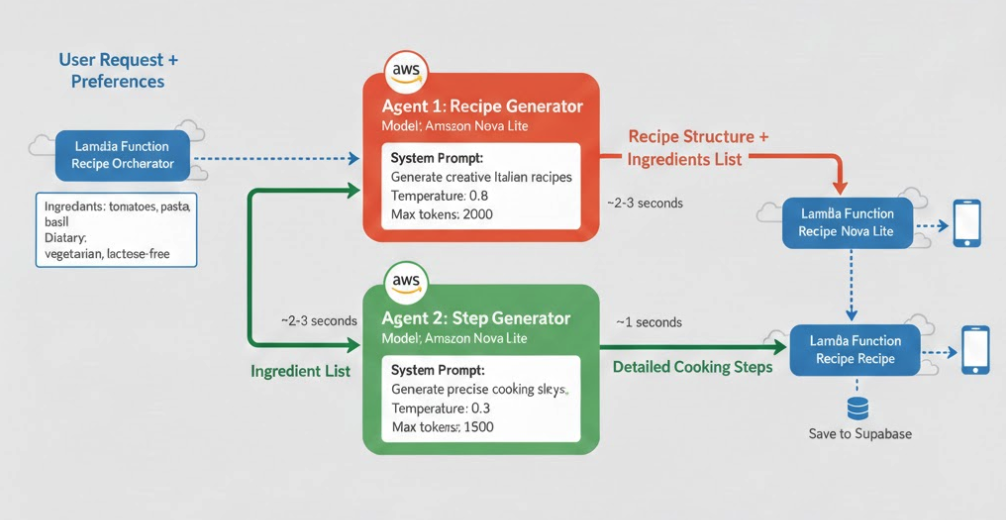
\includegraphics[width=0.85\linewidth]{Images/full_steps_aws.png}
% 	\caption{Flusso di generazione ricetta + passaggi preparazione}
% 	\label{fig:aws_serverless_architecture}
% \end{figure}

% \section{Sicurezza e Gestione Identità: AWS IAM}
% \label{sec:aws-iam}

% \subsection{Security by Design: Il Principio del Privilegio Minimo}

% La sicurezza in un sistema che gestisce dati personali sensibili come preferenze alimentari, obiettivi di salute e abitudini nutrizionali non può essere un'aggiunta successiva o un ripensamento, ma deve essere integrata nel design fin dal primo giorno. AWS Identity and Access Management (IAM)~\cite{aws_iam} è il servizio che controlla l'accesso a tutte le risorse AWS, e nel nostro sistema è stato applicato rigorosamente il \emph{principio del privilegio minimo}: ogni componente, che si tratti di una funzione Lambda, di un utente umano, o di un ruolo di servizio, riceve solo ed esclusivamente i permessi strettamente necessari per svolgere il proprio compito, niente di più.

% Questo approccio di ``security by design'' crea una difesa in profondità: anche se un attaccante riuscisse a compromettere un singolo componente del sistema, il danno sarebbe contenuto in un perimetro ristrettissimo. Concretamente, questo significa che la funzione Lambda responsabile di generare ricette può invocare l'agente Bedrock specificamente creato per questo scopo, e può scrivere log nel gruppo CloudWatch dedicato alla sua funzione. Ma non può fare altro: non può accedere ad altri agenti Bedrock, non può leggere i log di altre funzioni, non può modificare configurazioni di sistema, non può accedere al database Supabase direttamente. Ogni permesso deve essere esplicitamente concesso tramite una policy IAM.

% Un esempio concreto dalla nostra implementazione chiarisce questo concetto. La policy IAM associata alla funzione Lambda di generazione ricette è strutturata come mostrato nel Listing~\ref{lst:iam-policy-example}. Questa policy, scritta in formato JSON, specifica esattamente due permessi: il primo consente di invocare l'agente Bedrock con l'identificativo specifico del nostro agente di generazione ricette (e solo quello), il secondo permette di creare e scrivere log nel gruppo CloudWatch specifico di questa funzione. Qualsiasi altra azione su qualsiasi altro servizio AWS viene implicitamente negata.

% \begin{lstlisting}[language=json, label=lst:iam-policy-example]
% {
%   "Version": "2012-10-17",
%   "Statement": [
%     {
%       "Effect": "Allow",
%       "Action": "bedrock:InvokeAgent",
%       "Resource": "arn:aws:bedrock:eu-west-1:123456789012:agent/AGENTID/recipe-agent"
%     },
%     {
%       "Effect": "Allow",
%       "Action": "logs:CreateLogGroup",
%       "Resource": "arn:aws:logs:*:*:log-group:/aws/lambda/recipe-generator"
%     }
%   ]
% }
% \end{lstlisting}
% \noindent\footnotesize\textit{Nota: gli ARN riportati utilizzano valori placeholder
% (\texttt{123456789012} per l'account ID, \texttt{AGENTID} per l'identificativo
% dell'agente) in sostituzione dei valori reali per ragioni di sicurezza.
% Nella configurazione effettiva, ogni campo è sostituito dall'identificativo
% specifico della risorsa, in accordo con il principio del privilegio minimo.}
% \normalsize

% \subsection{Ruoli, Trust Policies e Segregazione}

% Ogni funzione Lambda nel nostro sistema opera sotto l'identità di un \emph{ruolo IAM} dedicato. A differenza degli utenti IAM (che rappresentano persone o applicazioni con credenziali permanenti), i ruoli sono identità temporanee che possono essere ``assunte'' da servizi o applicazioni per un periodo limitato. Le \emph{trust policy} definiscono esattamente quali entità possono assumere un determinato ruolo. Nel caso delle nostre funzioni Lambda, la trust policy specifica che solo il servizio Lambda di AWS può assumere quel ruolo, e solo per eseguire quella specifica funzione.

% Questa architettura basata su ruoli offre diversi vantaggi di sicurezza significativi. Innanzitutto, le funzioni non hanno accesso a risorse non esplicitamente autorizzate, creando confini di sicurezza netti tra i diversi componenti del sistema. In secondo luogo, in caso di compromissione di una singola funzione (ad esempio, tramite una vulnerabilità nel codice), il danno potenziale è limitato al perimetro di quella specifica funzione e ai permessi del suo ruolo associato. Un attaccante che compromettesse la funzione di generazione ricette non potrebbe, ad esempio, accedere ai dati di autenticazione degli utenti o modificare altre funzioni del sistema. Infine, l'audit e il monitoring sono enormemente semplificati: ogni azione eseguita nel sistema AWS viene tracciata e loggata con l'identificativo del ruolo che l'ha compiuta, creando una traccia di audit completa e immutabile che può essere analizzata per scopi di sicurezza, compliance o debugging.

% \section{Monitoraggio e osservabilità: AWS CloudWatch}
% \label{sec:aws-cloudwatch}

% Uno dei grandi problemi delle architetture serverless è l'invisibilità intrinseca: non esiste un server fisico o virtuale a cui connettersi tramite SSH per vedere cosa sta succedendo in tempo reale. Le funzioni Lambda nascono, eseguono il loro compito in pochi secondi o millisecondi, e poi scompaiono senza lasciare traccia. Come si fa a capire se il sistema sta funzionando correttamente? Come si diagnostica un problema quando un utente riporta che la generazione di una ricetta è fallita? Come si ottimizzano le performance quando non si può ``guardare dentro'' i server?

% AWS CloudWatch~\cite{cloudwatch} è la risposta a queste domande. È il servizio di monitoraggio e osservabilità di AWS che trasforma l'oscurità di un'architettura serverless distribuita in trasparenza operativa. Tutte le funzioni Lambda, automaticamente e senza configurazione aggiuntiva, inviano i loro log a CloudWatch. Ogni invocazione di un agente Bedrock viene tracciata. Ogni richiesta che passa attraverso API Gateway lascia una traccia. Questo crea un registro completo e immutabile di tutto ciò che accade nel sistema, con timestamp precisi al millisecondo e contesto completo per il debugging.

% Per il sistema di Cucina Generativa, è stato configurato il monitoraggio di metriche chiave che ci permettono di mantenere alta la qualità del servizio. La latenza di Bedrock misura il tempo che impiega il modello AI a generare una risposta completa: impostando una soglia di alert a cinque secondi, oltre la quale l'admin di sistema riceve una notifica per investigare possibili problemi di performance. Il tasso di errori Lambda traccia la percentuale di invocazioni che terminano con un'eccezione o un errore: una soglia dell'uno percento attiva un alert che richiede intervento immediato. Il conteggio dei token utilizzati per ogni ricetta generata ci permette di monitorare i costi operativi in tempo reale e di ottimizzare i prompt per ridurre il consumo senza compromettere la qualità. Infine, il tasso di successo end-to-end misura la percentuale di ricette generate correttamente e validate rispetto al totale delle richieste, fornendo una metrica di qualità del servizio dall'alto livello.

% \subsection{Alerting Proattivo e Visualizzazione}

% CloudWatch non si limita a raccogliere dati passivamente: permette di configurare alert basati su metriche, soglie e anomalie rilevate automaticamente. Ad esempio, configurando un alert che si attiva quando la latenza al novantacinquesimo percentile (P95) delle chiamate a Bedrock supera i cinque secondi per più di tre minuti consecutivi. Questo tipo di monitoring proattivo ci permette di rilevare e risolvere problemi prima che diventino evidenti agli utenti.

% Inoltre, CloudWatch Dashboards ci permette di creare visualizzazioni personalizzate dello stato di salute del sistema in tempo reale. La dashboard principale del sistema di Cucina Generativa mostra grafici temporali delle invocazioni Lambda per ora del giorno, la distribuzione della latenza Bedrock, il tasso di errori aggregato, e il costo stimato in tempo reale basato sul consumo di servizi. Questa visibilità è fondamentale per diversi motivi: consente di rilevare anomalie e problemi proattivamente prima che impattino significativamente gli utenti, fornisce dati concreti per ottimizzare performance e costi basandosi su pattern d'uso reali anziché su supposizioni, e offre trasparenza sull'utilizzo del sistema a tutto il team, facilitando discussioni informate su priorità di sviluppo e allocazione di risorse.

% \begin{figure}[H]
% 	\centering
% 	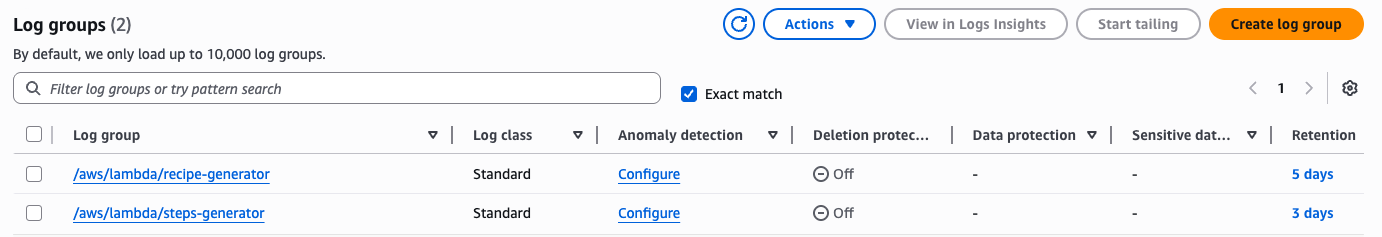
\includegraphics[width=1\linewidth]{Images/log_groups.png}
% 	\caption{Log Groups per gli endpoint Lambda}
% 	\label{fig:cloudwatch_dashboard}
% \end{figure}

% \section{Integrazione con l'Ecosistema Esistente}
% \label{sec:integrazione-ecosistema}

% \subsection{Un'Architettura Ibrida: Il Meglio di Due Mondi}

% Una delle decisioni architetturali più importanti del progetto è stata quella di adottare un approccio ibrido, combinando i punti di forza di Supabase per la gestione dei dati strutturati con la potenza dei servizi AI di AWS. Questa scelta merita una spiegazione approfondita perché rappresenta un bilanciamento attento tra diversi requisiti tecnici e di business.

% Supabase rimane il database primario del sistema per diverse categorie di dati. I profili utente, inclusi dati anagrafici, preferenze alimentari salvate, obiettivi nutrizionali e storico delle ricette generate, risiedono in PostgreSQL gestito da Supabase. Il database degli ingredienti e degli alimenti, con i relativi valori nutrizionali dettagliati (calorie, proteine, carboidrati, grassi, vitamine e minerali), è anch'esso memorizzato su Supabase per facilitare query complesse e relazioni tra entità. Infine, l'autenticazione e la gestione delle sessioni utente vengono gestite interamente da Supabase Auth, che fornisce token JWT validati poi da API Gateway.

% Questa architettura ibrida combina i punti di forza di entrambe le piattaforme in modo sinergico. Supabase offre semplicità e rapidità di sviluppo, con un'interfaccia intuitiva per la gestione del database, autenticazione pronta all'uso, e real-time subscriptions per aggiornamenti live. AWS, d'altra parte, fornisce la potenza computazionale e i servizi di intelligenza artificiale necessari per la generazione delle ricette, insieme a strumenti enterprise di monitoraggio, sicurezza e scalabilità.

% Un aspetto cruciale di questa scelta è la conformità al GDPR. Supabase permette di deployare i database in datacenter europei, garantendo che i dati personali degli utenti (informazioni sensibili come abitudini alimentari e obiettivi di salute) rimangano fisicamente nell'Unione Europea, come richiesto dalla normativa sulla privacy. L'elaborazione AI su AWS, invece, può avvenire in region diverse (come us-east-1 dove Bedrock ha la maggiore disponibilità di modelli) perché i dati processati sono anonimi e temporanei: il prompt inviato a Bedrock non contiene informazioni identificative dell'utente, solo requisiti nutrizionali e preferenze generiche.

% \subsection{Comunicazione Sicura Tra Ecosistemi}

% La comunicazione tra l'applicazione mobile (che comunica principalmente con Supabase) e i servizi AWS di generazione ricette avviene attraverso un percorso sicuro e ben definito. API Gateway funge da punto di ingresso pubblico, esponendo endpoint HTTPS accessibili dall'applicazione mobile. L'autenticazione avviene tramite validazione di token JWT \cite{jwt_token} emessi da Supabase Auth: quando un utente effettua il login tramite l'app, Supabase genera un JWT firmato che l'app include in ogni richiesta ad API Gateway. Un Lambda Authorizer personalizzato valida il token, verifica la firma, controlla la scadenza, e autorizza o nega l'accesso agli endpoint protetti.

% Infine, tutti i dati in transito sono cifrati end-to-end tramite TLS 1.3, garantendo che anche in caso di intercettazione del traffico di rete, i dati rimangano illeggibili.

% Questa integrazione attentamente progettata permette di mantenere i dati utente sensibili nel database Supabase in Unione Europea per compliance GDPR \cite{compliance}, mentre l'elaborazione AI computazionalmente intensiva avviene su AWS sfruttando Bedrock e Lambda, creando un sistema che è al tempo stesso conforme alle normative, performante ed economicamente sostenibile.


% In conclusione, l'infrastruttura tecnologica del sistema di Cucina Generativa rappresenta un esempio di architettura moderna che bilancia scalabilità, sicurezza, costi e velocità di sviluppo. La scelta di AWS come piattaforma serverless per l'elaborazione AI, integrata con Supabase per la gestione dei dati strutturati, crea un sistema robusto e flessibile. L'applicazione rigorosa di principi di sicurezza come il privilegio minimo tramite IAM, il monitoraggio continuo tramite CloudWatch, e l'uso di modelli AI ottimizzati come Nova Lite su Bedrock, garantisce che il sistema possa servire gli utenti di Builtdifferent con ricette personalizzate di alta qualità, mantenendo al contempo costi operativi sostenibili e piena conformità alle normative sulla privacy. Nei capitoli successivi, vedremo come questi componenti infrastrutturali vengono orchestrati per implementare il flusso completo di generazione ricette, dalla richiesta dell'utente alla consegna della ricetta personalizzata.